\section{Pojačano učenje}
Najistaknutije osobine pojačanog učenja su pokušaj i neuspjeh, te odgođena nagrada koje algoritam doživljava u okruženju. Algoritam bi trebao, do neke razine, imati osjećaj i informacije o okolini, te cilj ili cilevi prema kojima teži, a odnose se na određeno stanje u okolini.

\subsection{Povijest pojačanog učenja}
---> POVJEST ODE <---

\subsection{Elementi pojačanog učenja}
Osnovni građevni blokovi na kojem se temelju metode pojačanog učenja su:
\begin{itemize}
	\item Polica: Opisuje ponašanje u određenom trenutku. Određuje koje radje poduzeti ovisno o stanju okruženja, iskazuje se kao funkcija vjerojatnosti koja opisuje vjerojatnost sljedeće određene radnje.
	
	\item Signal nagrade: Govori algoritmu koliko je uspješan i primarni cilj svakog algoritma pojačanog učenja je težiti prema najvećoj mogućoj nagradi. 
	
	\item Funkcija vrijednosti: Daje određenoj situaciji konkretnu vrijednost. Na neki način procjenjuje buduću nagradu, što ga čini sekundarnim ciljem algoritmu pojačanog učenja. Uspješnim predviđanjem dugoročne nagrade poboljšava i ubrzava process izvršavanje primarnog cilja. 
	
	\item Model okruženja: Neobavezni element, koji oponaša okruženje. Pomaže algoritmu planirati buduća ponašanja. Algoritmi koji se služe modelom nazivaju se metode bazirane na modelu (eng. \textit{Model based}) za razliku jednostavnijim metodama slobodni od modela (eng. \textit{Model free}).
\end{itemize}

\subsection{Konačan Markov proces odlučivanja}
Formalizacija sekvencijalnog postupka donošenje odluka u kojima se uključuje, osim neposredne nagrade, odgođena nagrada. Procjenjuje se vrijednost za svaku radnju u nekom stanju $q_*(s,a)$ ili vrijednost stanja $v_*(s)$. 

Osnovni elementi su:
\begin{itemize}
	\item Agent
	\item Okruženje
	\item Stanje
	\item Akcija
	\item Nagrada
\end{itemize}

Svaka okolina se sastoji od skup stanja $S$ te definira dozvoljene akcije $A$. Osim toga još mora na neki način opisati nagrade $R$. Skupovi $S$, $A$ i $R$ se smatraju konačnim, te za svaki korak $t=0,1,2,...$ u okruženju, agent doživljava stanje $S_t \in S$ i bira akciju $A_t \in A$.


U markovom procesu odlučivanja (eng. \textit{Markov decision process}) se definiraju skupovi za stanja $S$, akcije $A$ te nagrade $R$. Svi skupovi se smatraju konačnim, te u svakom vremenskom koraku $t = 0, 1, 2, ..$, agent proučava stanje $S_t \in S$. U svakom vremenskom koraku pridružena akcija stanju daje par $(S_t, A_t)$, te izvršavanje agentovu radnju okruženje prelazi u sljedeće stanje $S_t+1 \in S$. U novom stanju agent primi nagradu $R_t+1 \in R$ i proučava novo stanje kako bi primjenio sljedeću akciju. Ovaj proces se može opisati funkcijom $f(S_t, A_t) = R_t+1$, te interakcija agenta i okruženja prikazana je na slici~\ref{fig:mdp_diagram}.
\\[\intextsep]
\begin{minipage}{\linewidth}
	\centering%
	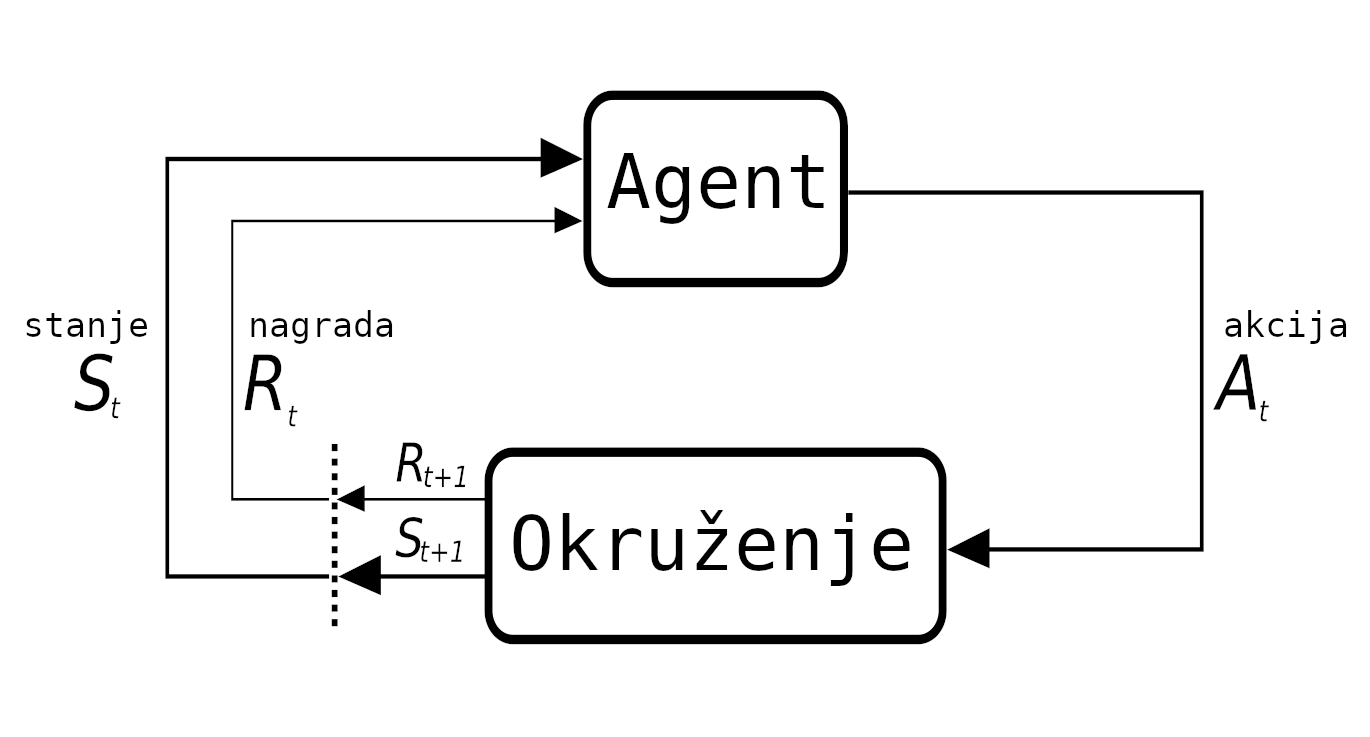
\includegraphics[width=0.8\linewidth,clip=]{images/mdp_diagram.png}%
	\figcaption{Diagram markovog procesa odlučivanja}%
	\label{fig:mdp_diagram}%
\end{minipage}
\\[\intextsep]

\subsection{Nagrada}
Očekivana nagrada $G_t$ se računa kao zbroj svih budućih nagrada $G_T = R_{t+1}+R_{t+2}+R_{t+3}+ ... + R_T$, gdje $R_T$ predstavlja nagradu u konačnom stanju okruženja. Prolaženjem jednom od početnog stanja do krajnog naziva se \emph{epizoda}, tako da pokretanje nove epizode okruženje se ponovno namjesti na neko određeno stanje neovisno o tome kako je prijašna epizoda završila. Međutim kako je agentu važnija neposredna nagrada, a osim toga postoje okruženja u kojima se neprekidno prelazi iz stanja u stanja i okruženje ne posjeduje konačno stanje, uvodi se pojam \emph{popust budućih nagrada}. Tako da za svaku sljedeću buduću nagradu uzme sve manje u obzir. Ovakva očekivana nagrada se definira kao $R_{t+1} + \gamma R_{t+2} + \gamma ^2 R_{t+3}+...$, gdje gamma predstavlja stopu popusta budućih nagrada, $0 \leq \gamma \leq 1$, tako da sada $G_T$ opisan jednadžbom~\ref{eq:suma_budućih_nagrada_s_popustom}.
\begin{equation}\label{eq:suma_budućih_nagrada_s_popustom}
	G_T = \sum_{k=0}^{\infty} \gamma^k R_{t+k+1}
\end{equation}

\subsection{Police i funkcije vrijednosti}
Polica određuje agentov sljedeći potez, kroz skupljanje iskustva ta polica se može mijenjati. Označava se sa $\pi$ i definira distribuciju vjerojatnosti preko $a \in A(s)$ za svaki $s \in S$, tako da konačne vjerojatnosti svake akcije $a = A_t$ u stanju $s = S_t$ opisane su policom $\pi(a|s)$.
Za opisivanje agentu dali se nalazi u dobrom stanju ili opisivanje agentu koliko je dobra akcija za neko stanje zadužene su funkcije vrijednosti. Koliko je dobro stanje, odnosno koliko je dobra neka akciju u nekom stanju agentu se daje do znanja pomoću vrijednosti očekivane nagrade. Funkcije vrijednosti se definiraju u odnosu na policu, pošto ona utječe na donošivanje agentove odluke.
Jedna od funkcije vrijednosti je funkcija vrijednosti stanja i pomoću nje agent dobije informaciju o očekivane nagrade, dok prati policu $\pi$, počevši od stanja $s$ u trenutku $t$. Formalno se označava matematičkom jednadžbom~\ref{eq:state_value_function}.
\begin{equation}\label{eq:state_value_function}
	\begin{split}
		v_\pi(s) &= \mathbb{E}_\pi[G_t | S_t = s] \\
				 &= \mathbb{E}_\pi\left[\sum_{k=0}^{\infty} \gamma^k R_{t+k+1} | S_t = s\right]
     \end{split}
\end{equation}
S druge strane postoji funkcija vrijednosti akcija $q_\pi(s, a))$ koja opisuje koliko je dobra akcija $a$ u stanju $s$ dok se prati polica $\pi$. Tako da funkcija računa vrijednost očekivane nagrade za svaku akciju i definirana je matematičkom jednadžbom~\ref{eq:action_value_function}.
\begin{equation}\label{eq:action_value_function}
\begin{split}
q_\pi(s, a) &= \mathbb{E}_\pi[G_t | S_t = s, A_t = a] \\
&= \mathbb{E}_\pi\left[\sum_{k=0}^{\infty} \gamma^k R_{t+k+1} | S_t = s, A_t = a\right]
\end{split}
\end{equation}
Slovo $q$ opisuje kvalitetu (eng. \textit{quality}) određene akcije i često se vrijednost naziva q-vrijednost, te funkcija koja je daje q-funkcijom. U jednadžbama~\ref{eq:state_value_function} i ~\ref{eq:action_value_function} $\mathbb{E}_\pi$ definira očekivanu vrijednost, u ovom slučaju očekivanu nagradu, slučajne variable praćenjem police $\pi$.

\subsubsection{Optimalne police i funkcije vrijednosti}
Jedna od osnovnih značakih pojačanom učenju koja se ističe, je da algoritam ima neki definirani cilj, prema kojemu teži. Glavni cilj je pronalaženje optimalne police, koju će agent pratit, kako bi doveo nagradu do najveće moguće razine. Neka polica $\pi$ se smatra boljom od neke druge police $\pi'$, ili bar jednako dobro, ako za sva moguća stanja nudi višu, ili jednaku nagradu za agenta. Optimalna polica je je ona koja za sva moguća stanja daje najveću nagradu i kada ne postoju neka druga polica koja za neko stanje daje veću nagradu. Također optimalna polica posjeduje njoj pripadajuću optimalnu funkciju vrijednosti stanja, odnosno optimalnu funkciju vrijednosti akcija. Optimalne funkcije se bilježe $v_*$ gdje $v_*(s) = \max_\pi v_\pi(s)$ za funkciju vrijednosti stanja, a za funkcije vrijednosti akcija $q_*$ gdje $q_*(s, a) = \max_\pi q_\pi(s, a)$ i to za sva $s \in S$, te u slučaju funkcije vrijednosti akcija još i za sva $a \in A$.

\subsection{Bellmanova jednadžba optimalnosti}
U nastavnom djelu ovoga rada usredočenje će biti na $q_*$, tako da se $v_*$ neće razrađivati. To ne znači da to nije primjenivo za $v_*$, ali izrada agenta ide u smjeru q-učenje (eng. \textit{q-learning}), pa je sav daljan opis prilagođen za to. 
Po Bellmanovoj jednadžbi, koju bi trebao svaki algoritam kojemu je cilj pronalaženje optimalne funkcije vrijednosti zadovoljiti, svaka očekivana nagrada jednaka je trenutačnoj nagradi dodana na maksimalne buduće nagrade sa popustom. Ima za zadatak pronaći $q_*$ koja zadovoljava jednadžbu~\ref{eq:bellman_optimality_equation}.
\begin{equation}\label{eq:bellman_optimality_equation}
q_*(s, a) = \mathbb{E}\left[R_{t+1} + \gamma\max_{a'}q_*(s', a')\right]
\end{equation}
Trenutačno stanje i akcija predstavljeni su sa $s$ i $a$, iz koji proizlazi nagrada $R_{t+1}$. Pa je toj nagradi za bilo koje buduće stanje $s'$ i buduće akcije $a'$ dodana vrijednost maksimalne buduće nagrade sa popustom. Pošto se donosi optimalnu akciju u stanju $s$, očekuje se da će se u sljedećemu stanju $s'$ moći izvršiti optimalnu akciju $a'$.

\subsection{Q-Učenje}
Ideja q-učenju jest tablica u kojoj je svaki redak određeno stanje u okolini, a svaki stupac određena akcija za tu okolini. Tako da u svakoj ćeliji se nalazi q-vrijednost za odeđenog para stanja i akcije. Početne q-vrijednosti postavljene su na nulu, jer agent još nije posjetio niti jedno stanje i nema ikakvih informacija o okolini. Prolaženjem kroz stanja okoline i izvršavanje akcije se te q-vrijednosti ažuriraju, tako da češćem izvršavanjem iste akcije u nekom stanju ta q-vrijednost se sve više približava stvarnoj. Pošto tablica u početku nema korisnih informacija o tome koje akcije poduzeti uvodu se pojmove istraživanja (eng. \textit{exploration}) i iskorištavanje (eng. \textit{exploitation}). Gdje u fazi istraživanja agent donese nasumičnu odluku, tako da u sljedećemu stanju primi nagradu i ovisno o tome može ažurirati q-vrijednost u tablici. Istraživanje služi za prikupljanje informacije o okolini kako bi se u buduće moglo donijeti što bolju odluku. U fazi iskorištavanja agent izvrši po njemu najbolju akciju, odnosno pronađe redak u q-tablici koji odgovara trenutačnom stanju i ovisno o tome koja akcija sadrži najvišu q-vrijednost, ta je akcija izabrana. A ta faza služi za prikupljanje najviše moguće nagrade, što je ipak i agentov glavni zadatak.

\subsubsection{Epsilon pohlepna strategija}
Potreban je neki omjer koji raspoređuje koliko i kada će se istraživati, odnosno iskorištavati. Želi se izbjeći istraživanje kada se posjeduje dovoljno informacija o okolini i izostat maksimalnoj nagradi, a također se želi izbjeći iskorištvati sa nedovoljno informacija o okolini, što isto tako dovodi do neuspješnog prikupljanje maksimalne nagrade. Taj omjer u epsilon pohlepnoj strategiji (eng. \textit{epsilon greedy strategy}) je $\epsilon$ i broj je između 0 i 1. Odluka se donosi na način da se nasumično generira broj između 0 i 1, te ako je taj broj veći od $\epsilon$ onda se iskorištava, znači izabere se akcija koja bi trebala donjeti najvišu nagradu, ako je manji onda se istražuje i izvrši se nasumična akcija. Što dovodi do zaključka da sa $\epsilon = 1$ je 100\% sigurno da će se istraživati a kada je $\epsilon = 0$ se neće nikako. Kako se situacije razlikuju dali agent posjećuje svoje prvo stanje ili je već neko vrijeme proveo u okolini i prošao dosta stanja, se prema tome mora i prilagoditi $\epsilon$. Za prilagođavanje koristi se stopa propadajućeg epsilona (eng. \textit{epsilon decay rate}), tako da na početku je $\epsilon = 1$ i vremenom opada i sve više se približava 0. Znači da je na početku agentu veći prioritet iztraživati okolinu i vremenom sve više i više iskorištava. Po terminologiji algoritama se smatra nekim algoritmom \emph{pohlepnim} kada uzme u obzir samo neposrednu vrijednost, odnosno nagradu, u obzir bez da se razmatra dugoročne posljedice. Pa se zbog toga kaže da agent vremenom postane pohlepan. Najčešće se $\epsilon$ nikad ne desegne vrijednost nule, nego ga se prestane smanjivati u trenutku kada $\epsilon = 0.1$, tako da u 10\% skučajeva agent i dalje istražuje, kako mu nebi nešto promaklo.

